\section{Modeling}

\begin{figure}[htbp]
    \centering
    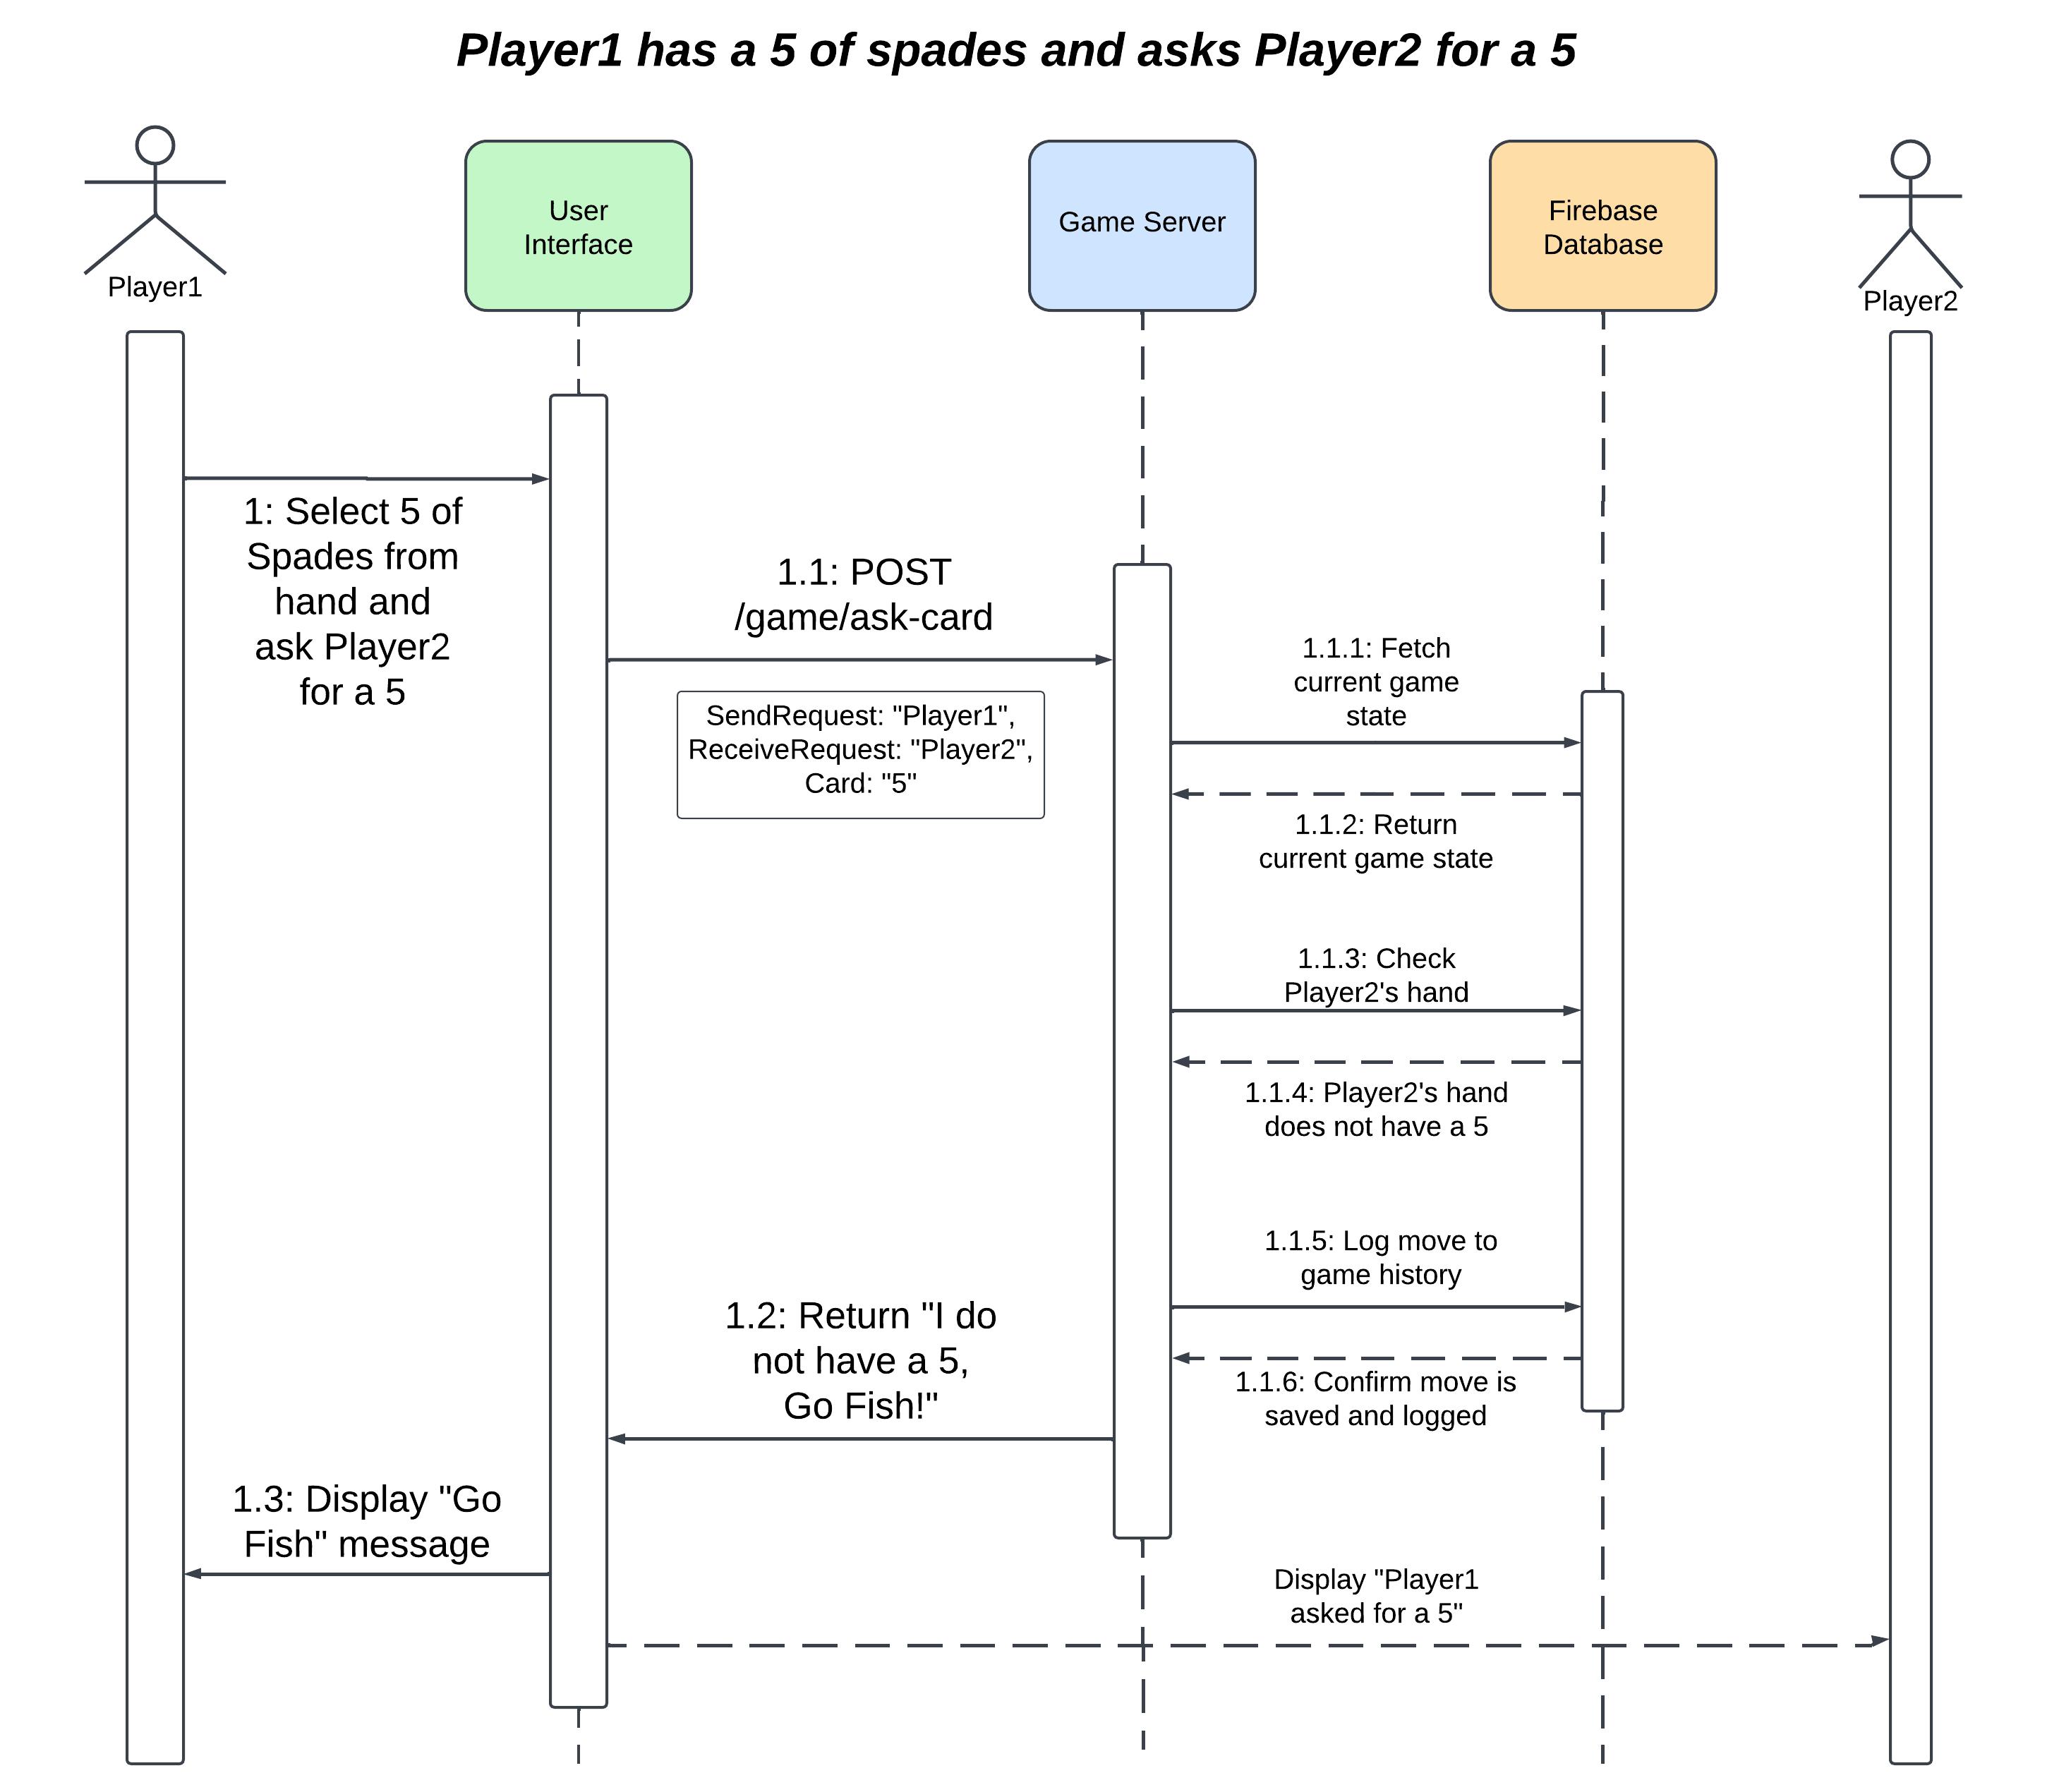
\includegraphics[width=1\linewidth]{CS482 Sequence Diagram Sprint 2.png}
    \caption{UML sequence diagram of Player1 asking for a card that they have in their hand, Player2 does not have this card, and thus Player1 is told to "Go Fish"}
    \label{fig:umlsequence}
\end{figure}

This UML sequence diagram visualizes a key aspect of our gameflow. When it is a player's turn, they first select a card in their hand. In this case, Player1 has a 5 of Spades in their hand. Then, they must ask another player if they have their card in their hand. Specifically the rank, but since Player2 does not possess a 5 in their hand, Player2 cannot give up any card in their hand.

In the diagram, the server sends a request to the database for data on Player2's hand. Then, a response is sent back which contains Player2's cards. There is then a check done between Player1's hand and Player2's hand for if Player2 has a 5, which they do not, so then no card is taken from Player2. Thus, this move is logged and the game returns "Go Fish!" to Player1.